
\chapter{Implementation of the~Proposed Evaluation Methods}
\label{chapter-5}
This chapter describes the~implementation of the~two evaluation techniques proposed in Section~\ref{comparison-methods-label}. The~two evaluations are implemented as a~single, comprehensive evaluation. The~source code is available on GitHub\footnote{\url{https://github.com/Aenariss/DIP}}. The~chapter outlines the~technologies used and describes the~implementation logic. In this chapter, various limitations are mentioned. Additional limitations are presented in Chapter~\ref{limitations-chapter}.

To support comparison of privacy-oriented browsers, such as the~Avast Secure Browser, which is available only on \textit{Mac} and \textit{Windows} desktop operating systems, \textit{Windows 11} was selected as the~operating system for the~evaluation of the~content-blocking tools. Docker was not used to containerize the~system since running a~Windows OS inside a~Docker is not officially supported. Instead, the~implementation can be run natively on a~Windows machine or within the~included virtual environment, provided the~host machine supports nested virtualization since Docker is utilized to run a~custom DNS server. The~implementation is written in Python\footnote{\url{https://www.python.org/}}, chosen for its easy access to many libraries.

Given the~objective of simulating user behavior, such as visiting web pages using a~browser with or without privacy-preserving extensions, \textit{Selenium} is employed for automation. Additional technologies used in the~evaluation are discussed in their respective sections. The~program can operate on either previously stored traffic or newly acquired data to ensure reproducibility and determinism across multiple evaluations. Figure~\ref{highlevel_overview}  depicts the~high-level overview of the~evaluation system.

\begin{figure}[!ht]
    \centering
    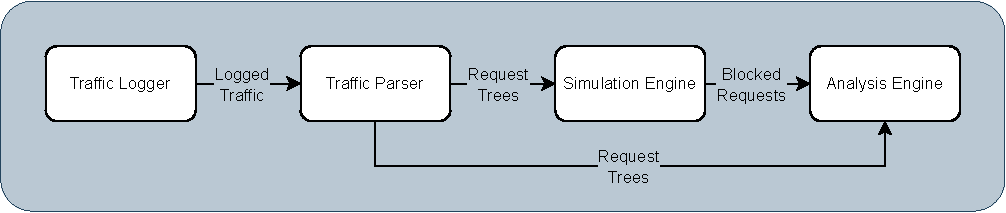
\includegraphics[width=\textwidth]{obrazky-figures/highlevel_overview.pdf}
    \caption[High-level overview of content-blocking tool evaluation system]{High-level overview of content-blocking tool evaluation system.}
    \label{highlevel_overview}
\end{figure}

The overview shows that the~system consists of four primary components, each independently executable. The~modularity ensures that the~system can, for example, be configured to collect traffic data without performing any subsequent parsing. 

\section{Traffic Logger}

The objective of the~traffic logger is to collect data from designated sites or to load previously gathered data. The~collected data for each page are \textit{network traffic}, \textit{fingerprinting API calls} and Domain Name System \textit{(DNS)\footnote{\url{https://www.ietf.org/rfc/rfc1035.txt}} responses}.

Logged network traffic allows the~evaluation of a~content-blocking tool's effectiveness by measuring the~number of blocked requests. Observed fingerprinting API calls are used to determine a~content-blocking tool's inherent anti-tracking capabilities. Additionally, DNS responses are utilized to ensure determinism.

Users can specify the~pages from which the~traffic logger should collect data to maximize configurability. The~collection process is performed for each specified page and consists of the~following steps:

\begin{itemize}
\setlength\itemsep{0em}
\item Start the~DNS Response Monitor to capture DNS responses.
\item Create a~Selenium-driven Google Chrome browser instance\footnote{Traffic logging could theoretically work with other Chromium-based browsers, but traffic logger is implemented to utilize Google Chrome}.
\item Load a~custom configuration of the~JShelter extension into the~browser.
\item Visit the~specified page and collect data for user-defined duration. If the~page fails to load within the~user-specified maximum time, skip it and continue with the~next.
\item Quit the~browser and the~DNS Response Monitor and save the~logged data.

\end{itemize}

\subsection{DNS Responses and Logs}
Logging DNS responses allows the~evaluation to save the~IP address and possibly \textit{CNAME}s associated with each request. This data can be utilized to repeat the~response later, ensuring determinism, since some content-blocking tools can use the~IP address associated with a~domain to block the~request\footnote{Tested with uBlock Origin 1.63.0~using a~custom filter in Firefox. Also tested in Brave Browser (Chromium-based) with the~same configuration -- only works in Firefox.}. The~DNS Monitor uses the~\textit{Scapy}\footnote{\url{https://scapy.net/}} Python module.

\subsubsection{CNAME Cloaking}
\label{cname-cloaking-implementation}
Another reason for logging DNS responses is to address the~issue of CNAME cloaking~\cite{cname-cloaking}. Figure~\ref{dns_resolution_ok} depicts how a~DNS resolution should proceed for domain \texttt{tracker.example.com}. Suppose our content-blocking tool includes a~rule that blocks \texttt{tracker.example.com}. In that case, the~content-blocking tool would block the~request before any DNS query could even be created.

\begin{figure}[!ht]
    \centering
    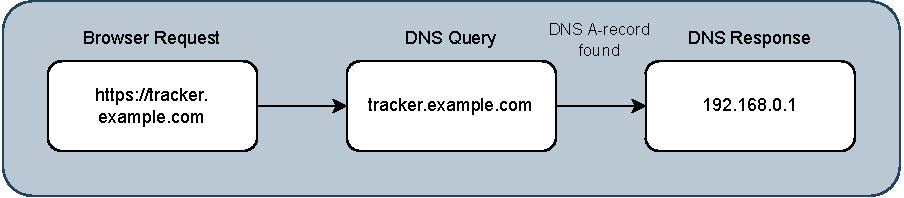
\includegraphics[width=\textwidth]{obrazky-figures/dns_resolution.pdf}
    \caption[DNS resolution with no CNAME records]{DNS resolution for domain \texttt{tracker.example.com} with no CNAME records present.}
    \label{dns_resolution_ok}
\end{figure}

To illustrate the~CNAME cloaking issue, suppose a~page requests data from domain \linebreak \texttt{not-a-tracker.example.com}. Under normal circumstances, the~DNS server would return an~\textit{A} record, as in the~previous Figure~\ref{dns_resolution_ok}. However, if a~CNAME record exists for the~domain instead of an~A record, the~resolution of \texttt{not-a-tracker.example.com} could, in reality, lead to \texttt{tracker.example.com}, which only then leads to the~A record. Figure~\ref{dns_resolution_cname} depicts this situation.

\begin{figure}[!ht]
    \centering
    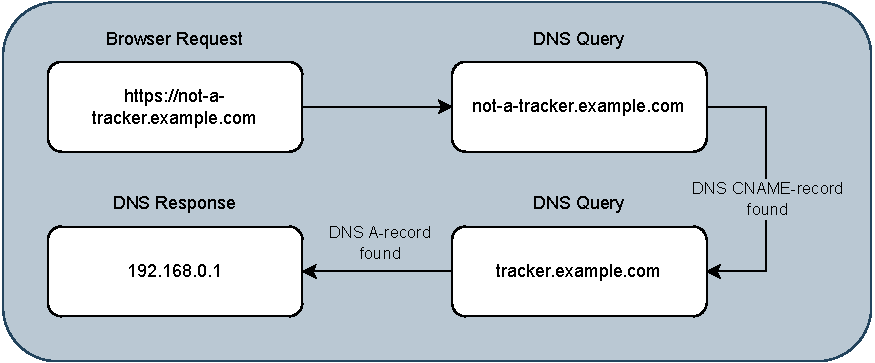
\includegraphics[width=\textwidth]{obrazky-figures/dns_resolution_cname.pdf}
    \caption[DNS resolution with CNAME records]{DNS resolution for domain \texttt{not-a-tracker.example.com} with a~CNAME record present.}
    \label{dns_resolution_cname}
\end{figure}

Suppose that the~tested content-blocking tool does not block \texttt{not-a-tracker.example.{\linebreak}com}, even though it resolves into the~unwanted \texttt{tracker.example.com}. If the~tool does not see the~intermediate step in the~resolution process, it does not block the~request. CNAME responses are logged to replicate these situations. To replicate the~DNS responses later, all A~and CNAME responses are stored for each domain and its subdomains. Examples of observed DNS responses are shown in Listing~\ref{stored-dns-figure} in Appendix~\ref{json-appendix}.


\subsection{Default JShelter Version}
As previously mentioned, JShelter is used to collect fingerprinting logs for each page. By default, JShelter includes functionality to protect users from browser fingerprinting. However, since this would affect visited sites, it must be disabled. 

In the~pre-compiled version of JShelter, fingerprinting API calls are only logged should the~user explicitly choose to do so. The~button to start the~logging is located inside a~submenu, which is located in the~extension menu. The~submenu location is shown in Figure~\ref{jshelter_fpd}. After activation, tracing the~callers causes a~page reload and the~submenu to populate with observed callers. 

\begin{figure}[!ht]
    \centering
    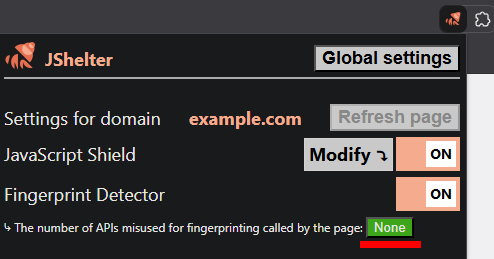
\includegraphics[scale=1.75]{obrazky-figures/jshelter_fpd.png}
    \caption[JShelter Fingerprint Detector button located in the~extension menu]{JShelter Fingerprint Detector button is located in the~extension menu. A~red line underscores the~button. The~menu must be opened to track callers of potentially fingerprintable APIs.}
    \label{jshelter_fpd}
\end{figure}

However, the~page reload breaks the~network logging. It leads to repeated entries in the~logs, making it difficult to distinguish the~original request tree. Additionally, if the~initially visited page redirects the~user to another page, the~reload only affects the~final page. Therefore, the~repeated network logs would be incomplete since the~original redirects would be lost.

Another issue with the~default version of JShelter is that it exposes the~caller data inside a~submenu, which can only be opened by manually clicking the~extension button. The~submenu location is shown in Figure~\ref{jshelter_fpd}. Since Selenium does not support interacting with extension menus\footnote{\url{https://github.com/seleniumhq/selenium-google-code-issue-archive/issues/7805}}, automating the~clicking process is not feasible.

\subsection{Custom JShelter Version}
\label{jshelter-custom-section}
I created a~custom version of JShelter 0.19~with all anti-tracking functionality disabled to address the~limitations of the~default JShelter version. In the~custom version, API caller tracking is enabled by default. Therefore, each time a~page is visited, JShelter automatically tracks the~callers by inserting the~required JavaScript wrappers and populating its internal callers list. To obtain the~fingerprinting data, JShelter is modified to automatically download a~JSON fingerprinting report \emph{five} seconds after a~page was accessed. Therefore, a~browser must remain on the~page for at least five seconds to successfully download the~report.

However, this approach has one severe limitation -- JShelter sometimes fails to insert the~wrappers correctly. The~issue is present only in Selenium, which is used to create the~dataset. It makes the~results in the~fingerprinting report empty. Testing with a~newer version of JShelter (0.20) resulted in an~even higher failure rate in the~Selenium environment. This ultimately led to using the~previous version 0.19.

Despite the~abovementioned limitation, the~JShelter Fingerprint Detector can still be used, albeit with limited results. Since all content-blocking tools are evaluated on the~same dataset, missing fingerprinting data for some pages is equivalent to those pages not using any fingerprinting API calls. That is, in turn, equivalent to a~smaller dataset being used.

\subsection{Network Logs}
I selected Google Chrome for traffic logging as it provides a~convenient way to obtain network logs. Network logs are later used to create request trees. For each specified page, a~new instance of Google Chrome is created and configured to log performance events\footnote{\url{https://developer.chrome.com/docs/chromedriver/logging/performance-log}}, including network logs. Listing~\ref{logging_code} shows the~command to enable performance logging.

\setcounter{listing}{0}
\begin{center}
    \begin{minipage}{\textwidth}
        \begin{lstlisting}[style=pythonstyle, label={logging_code}, caption={Command to configure the~browser to log performance events}]
chrome_options.set_capability("goog:loggingPrefs", {"performance": "ALL"})
        \end{lstlisting}
    \end{minipage}
\end{center}

Afterward, network logs are obtained by parsing each record and identifying whether it matches a~\texttt{Network.requestWillBeSent}\footnote{\url{https://chromedevtools.github.io/devtools-protocol/tot/Network/\#event-requestWillBeSent}} event. If the~record matches this event, the~traffic logger saves it. Internal browser requests (e.g., requests starting with \texttt{chrome://}) are not included. For each \texttt{requestWillBeSent} event, three key attributes are logged:

\begin{itemize}
\setlength\itemsep{0em}
\item \texttt{documentURL}, renamed as \texttt{requested\_for}: The~URL of the~document the~request is loaded for.
\item \texttt{request.url}, renamed as \texttt{requested\_resource}: The~URL of the~requested data.
\item \texttt{initiator}: The~entity that initiated the~request.
\end{itemize}

\section{Traffic Parser}
The traffic parser is responsible for reconstructing request trees from the~logged data. The~trees are created from the~\textit{fingerprinting logs} and \textit{network logs}. The~process is summarized in the~following steps:

\begin{itemize}
\setlength\itemsep{0em}
\item Load fingerprinting groups from the~JShelter FPD settings.
\item Retrieve all wrapped APIs from the~FPD settings and assign each API a~primary group. The~current implementation requires the~FPD logs to originate from a~Chro\-mium-based browser.
\item Parse fingerprinting logs for each visited site and count fingerprinting API calls of each resource. Assign the~fingerprinting API calls to the~primary groups.
\item Construct a~request tree for each network log. Assign fingerprinting API calls to each resource in the~tree.
\end{itemize}

\subsection{Fingerprinting Groups and APIs}
\label{fp-groups-apis}
The goal of parsing fingerprinting logs is to determine the~number of fingerprinting API calls caused by each resource. According to the~JShelter FPD groups configuration file\footnote{\url{https://pagure.io/JShelter/webextension/blob/main/f/common/fp\_config/groups-lvl\_0.json}, accessed on \DTMdisplaydate{2025}{03}{04}{-1}}, the~API calls are divided into three main groups. Information about the~group configuration and other parts of JShelter Fingerprint Detector is explained in great detail in the~original thesis by Marek Saloň~\cite{salon-mit}.

Each wrapped fingerprinting API belongs to a~specific group, but the~configuration file specifies many groups. If all groups were used as-is, the~fingerprinting results would be overly detailed and challenging to understand. Each main group has multiple associated subgroups, which may also have their own subgroups. To improve readability, only the~three main groups are used. These groups are:

\begin{itemize}
\setlength\itemsep{0em}
    \item  \textit{BrowserProperties}: APIs that use browser properties representing the~state of \linebreak the~browser, such as the~\textit{Navigator} object.
    \item \textit{AlgorithmicMethods}: APIs that need to be dynamically calculated, such as the~\textit{Canvas} API.
    \item \textit{CrawlFpInspector}: APIs identified by Iqbar et al.~\cite{iqbal2020fingerprintingfingerprinterslearningdetect} as mostly used for fingerprinting purposes. It consists of APIs from both previous categories and some new ones.
\end{itemize}

As mentioned, each wrapped API belongs to a~specific group. The~APIs are defined in the~JShelter FPD wrapper configuration. Each observed API's associated subgroup is changed to one of the~three primary groups. For example, the~API \texttt{Navigator.prototype.{\linebreak}userAgent} belongs to a~group \textit{NavigatorBasic}, which in turn belongs to the~primary group \textit{BrowserProperties}. Therefore, the~group assigned to this API is changed to \textit{BrowserProperties}. Should the~API also be included in the~\textit{CrawlFpInspector} category, this group, too, is associated with that API. This way, no group information is lost, only reduced.

The configuration for both groups and wrapped APIs was obtained directly from \linebreak the~JShelter project\footnote{\url{https://pagure.io/JShelter/webextension/blob/main/f/common/fp_config/}}. This ensures that future updates to JShelter FPD can be easily integrated by replacing the~configuration files. 

\subsection{Associating Fingerprinting API Calls to a~Resource}
For each fingerprinting API call, the~complete call stack is logged. However, only the~\emph{final caller} in the~call stack is used to associate a~call with a~resource. For example, if script \emph{A} calls script \emph{B}, which then calls script \emph{C}, and \emph{C} uses a~potentially fingerprintable API, this call is attributed to script \emph{C}.

\subsection{Request Trees}
Request trees are a~vital part of the~evaluation process since they facilitate the~transitive properties of the~evaluation. Request trees are created using both network and fingerprinting logs. The~trees have a~limitation, however. If a~resource is requested multiple times, duplicate nodes are created, which distorts the~analysis results. The~duplication issue is explained further in Section~\ref{request_tree_issues}. 

The process of associating fingerprinting statistics to each resource has already been discussed; the~statistics are assigned to the~corresponding node in the~tree. If a~resource is already present in the~tree, the~new node's fingerprinting API calls are assigned twice, distorting the~results further. Each node in the~tree has the~following attributes:

\begin{itemize}
\setlength\itemsep{0em}
    \item \texttt{resource}: The~resource URL represented by the~node.
    \item \texttt{children}: A~list of nodes requested by this resource.
    \item \texttt{fp\_attempts}: The~number of fingerprinting API calls made by this node.
    \item \texttt{blocked}: Whether this node was blocked by a~content-blocking tool. It is only used during the~analysis phase (described in Section~\ref{content_blocking_analysis_subsection}).
    \item \texttt{root\_node}: Whether the~node is a~\textit{root} node or not.
    \item \texttt{parents}: The~resources that requested this node.
\end{itemize}

The request trees are constructed using three attributes from network logs -- \texttt{requested\_{\linebreak}for}, \texttt{requested\_resource} and \texttt{initiator}. The~network logs are parsed chronologically. During the~construction process, two types of nodes can be observed, as illustrated in Figure~\ref{root_regular_nodes}, which represents a~real example\footnote{The initially accessed URL was \texttt{https://zpravy.idnes.cz} on \DTMdisplaydate{2025}{03}{12}{-1}. Part of the~observed structure was omitted, and URL addresses were shortened for clarity.}.

\begin{figure}[!ht]
    \centering
    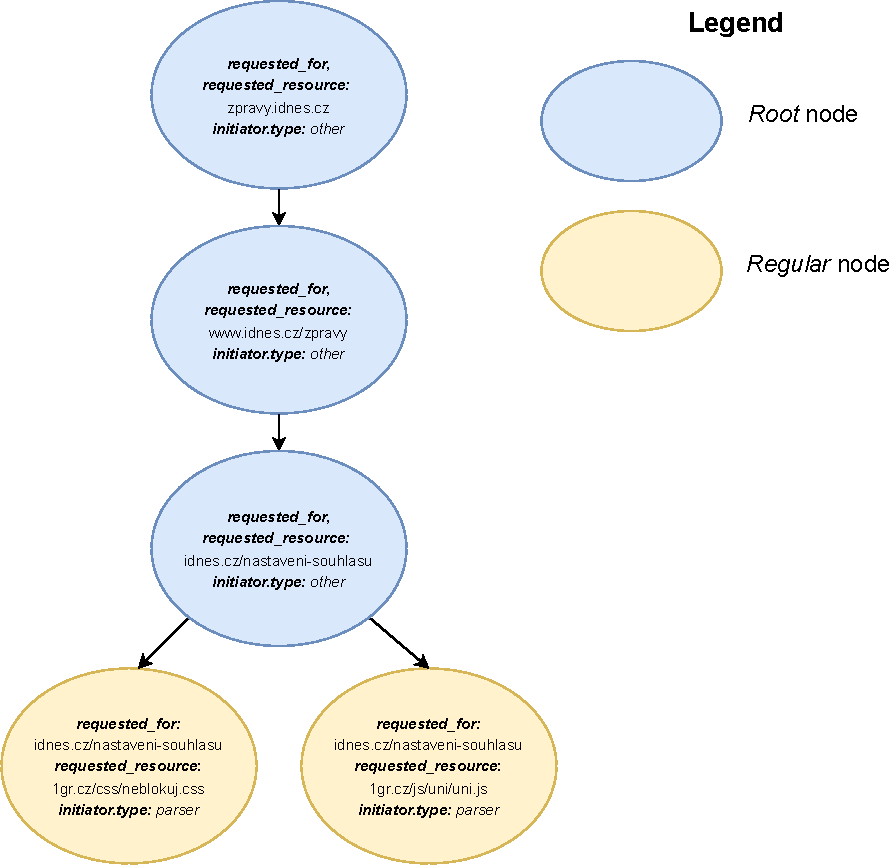
\includegraphics[scale=1]{obrazky-figures/root_regular_nodes.pdf}
    \caption[Illustration of \textit{root} and \textit{regular} nodes]{Illustration of \textit{root} and \textit{regular} nodes. For \textit{root} nodes, \texttt{requested\_resource} and \texttt{requested\_for} must match while also having \texttt{initiator.type} as \textit{other} and \texttt{initiator.url} not set. Regular nodes are all other nodes.}
    \label{root_regular_nodes}
\end{figure}

\subsubsection{Root nodes}
\label{root-nodes}
The \textit{root} nodes are characterized by the~\texttt{requested\_for} and \texttt{requested\_resource} attributes being identical and the~\texttt{initiator.type} being \textit{other}. \texttt{initiator.url} must also not exist. These nodes represent main pages loaded in the~browser (e.g., pages with URL shown in the~address bar), including any redirects leading to the~final page (i.e., the~page URL of which is shown in the~address bar). The~last node in the~sequence of \textit{root} nodes is used as the~parent node of all \textit{anonymous} nodes (i.e., the~nodes with no known parent). All unidentifiable fingerprinting API calls are also assigned to the~last \textit{root} node. 

\textit{Root} nodes have the~previous \emph{root} node set as their parent.
If no previous \textit{root} node exists, it was the~very first \textit{root} node observed -- in such case, the~node has no parent and represents the~root of the~whole tree. When one of the~\textit{root} nodes is loaded multiple times, i.e., two \texttt{Network.RequestWillBeSent} events have the~exact attributes \texttt{requested\_for}, \texttt{requested\_resource} and \texttt{initiator.type}, the~second such event is added as a~child of the~current \textit{root} node as a~\textit{regular} node. The~duplicate node has its associated fingerprinting API calls set to zero since they are already associated with the~primary node.

\subsubsection{Regular Nodes}
Any node that does not match the~specific characteristics of a~\textit{root} node is classified as a~\textit{regular} node. The~\textit{root} nodes have special parentage rules described above. The~traffic parser uses three methods to determine the~parentage of the~\textit{regular} nodes. However, the~first two methods described have a~limitation. Since the~trees may contain duplicate nodes, child nodes may be assigned to multiple parents, leading to redundant parent-child relations, which affect subsequent analysis.

\subsubsection{Initiator URL}
When the~attribute \texttt{initiator.url} is available, the~tree is searched for matching parent nodes (i.e., nodes with the~\texttt{resource} attribute matching this \texttt{initiator.url}).

\subsubsection{Initiator Call Stack}
When \texttt{initiator.url} is not available, the~final record of the~\textit{JavaScript} \textit{call stack} is utilized. Each record in the~call stack has \textit{url} specified, which represents the~URL of the~resource that caused the~event. Nodes representing this URL are selected as parents.

This approach has another limitation in addition to the~one described above. The~limitation is that calls may have come from a~dynamically generated code, such as from \textit{eval}\footnote{\url{https://developer.mozilla.org/en-US/docs/Web/JavaScript/Reference/Global_Objects/eval}}, which would show the~\textit{url} attribute as an~empty string. This situation is illustrated in Listing~\ref{empty_url_init}. It was caused by calling \textit{eval} as shown in Listing~\ref{eval_example_call}. In this case, the~call stack is traversed until a~valid URL is obtained. This URL is then set as the~parent, even though it may not reflect the~actual parent. The~current \textit{root} node is selected as the~parent if no valid URL exists.

\renewcommand{\thelstlisting}{\thechapter.\arabic{lstlisting}}
\renewcommand{\thelisting}{\thechapter.\arabic{listing}} 

\setcounter{listing}{1}

\begin{center}
    \begin{minipage}{\textwidth} % Adjust the~width as needed
        \begin{lstlisting}[style=pythonstyle, label={eval_example_call}, caption={Loading a~script using \textit{eval} which resulted in empty \textit{url} parameter in the~call stack.}]
eval("const script2 = document.createElement('script'); script2.src = '/script2.js'; document.body.appendChild(script2);")
        \end{lstlisting}
    \end{minipage}
\end{center}

\setcounter{listing}{2}
\begin{listing}[!ht]
    \begin{minted}[frame=none, breaklines]{json}
"initiator": {
    "stack": {
        "callFrames": [
            {
                "functionName": "eval",
                "url": ""
            },
            {
                "functionName": "",
                "url": "http://localhost:8000/script1.js"
            }
        ]
    },
    "type": "script"
}
    \end{minted}
    \caption{Example of empty \textit{url} attribute in the~call stack caused by the~use of \textit{eval}, which was called by \emph{script1.js}, but the~\empty{url} attribute of the~record does not reflect it. The~first record in the~list of call frames represents the~final call. This~presented call stack is edited and does not contain all logged attributes.}
    \label{empty_url_init}
\end{listing}

\subsubsection{Other}
If none of the~above is applicable, the~current \textit{root} node is selected as the~parent. In case a~valid parent could not be found for any reason (e.g. because an~\textit{iframe} with defined \texttt{srcdoc}\footnote{\url{https://developer.mozilla.org/en-US/docs/Web/API/HTMLIFrameElement/srcdoc}} property was opened, so the~\texttt{initiator.url} was specified as \texttt{about:srcdoc}), the~parent is also set as the~current \textit{root} node.


\section{Simulation Engine}
The simulation engine simulates which of the~requests from the~initial dataset would have been blocked by a~specified content-blocking tool. The~simulation attempts to partially replicate the~conditions of the~initial visit. To understand what requests a~given content-blocking tool would block, several steps are taken:

\begin{itemize}
\setlength\itemsep{0em}

\item Set up the~simulation. The~simulation includes a~custom DNS server to replicate DNS responses and a~custom web server to request all the~resources.
\item Configure a~client with the~content-blocking tool to be tested. Visit the~custom web server with the~client. 
\item Obtain results indicating what requests were blocked.

\end{itemize}

Each of these steps is described in greater detail in the~following subsections. The~simulation engine also creates firewall rules to prevent requests from leaving the~machine to save network bandwidth. 


\subsection{Custom DNS Server}
A custom DNS server is utilized to resolve DNS requests as they were observed to reproduce the~conditions present during the~initial visit. It allows the~tested tools to block requests depending on the~IP address to which they were resolved.
As mentioned in Subsection~\ref{cname-cloaking-implementation}, this step also allows the~tested tools to use methods allowing them to block requests utilizing CNAME cloaking. However, CNAME cloaking can only be prevented in Firefox since Chromium does not provide the~necessary API. 

I chose \textit{BIND 9\footnote{\url{https://www.isc.org/bind/}}} server for this purpose. It runs inside a~Docker container, built using an~existing image\footnote{\url{https://hub.docker.com/r/internetsystemsconsortium/bind9}}. To configure the~system to use the~custom DNS server as its default, the~\textit{Set-DnsClientServerAddress}\footnote{\url{https://learn.microsoft.com/en-us/powershell/module/dnsclient/set-dnsclientserveraddress}} Powershell command is executed from within the~program. After the~simulation ends, the~same command is used to reset Windows settings back to the~default state, using the~DNS server address provided by Dynamic Host Configuration Protocol \textit{(DHCP)} -- however, any custom configuration used before the~simulation launch is lost in the~process.

\subsubsection{Zone Files}
\textit{Zone}\footnote{\url{https://datatracker.ietf.org/doc/html/rfc1035}} files are used to define how domain names should be resolved. A~separate zone file is created for each observed second-level domain\footnote{e.g., for observed address \texttt{tracker.example.com}, zone file \texttt{example.com} is created, containing a~record for \texttt{tracker}. The~record can either be a~CNAME pointing to another domain or an~A record specifying an~IPv4 address.}. 

All DNS logs are merged to generate zone files correctly, and duplicates are removed. The~merging is possible since the~DNS responses remain valid for a~specified period of time. Therefore, during dataset creation, repeated DNS queries should return identical responses. However, a~DNS reply may have changed during dataset creation. The~merging erases this change, slightly limiting the~\textit{correctness} of DNS replies. 

If a~DNS response contains multiple IPv4 addresses, only the~\emph{first} address is used in the~zone file. This ensures that all queries for a~given domain are resolved into the~same address. Similarly, if a~response contains multiple CNAMEs, only the~first CNAME is added to the~zone file. However, no information is lost, as artificial records for all observed CNAMEs are present in the~logs. These artificial records ensure that every CNAME has its corresponding zone file, as illustrated in Listing~\ref{stored-dns-figure} in Appendix~\ref{json-appendix}\footnote{The accessed domain was \texttt{ads.pubmatic.com}. Response for this domain only was observed. The~other records were automatically added to be used with CNAMEs. Each of the~primary records will have its own zone file.}.

The simulation engine appends a~record to custom \texttt{named.conf} file for each zone file. \texttt{named.conf} is used to configure the~\textit{BIND 9} server to use the~created zone files. 
After all the~zone files are created and included in the~\texttt{named.conf}, the~zone files and the~\texttt{named.conf} are uploaded to the~Docker container, and the~server is restarted to apply the~changes.


\subsection{Custom Web Server}
The custom web server is responsible for repeating the~requests for all resources observed during dataset creation. \textit{Flask}\footnote{\url{https://flask.palletsprojects.com/en/stable/}} is used to build a~simple locally hosted webpage that dynamically loads recorded resources using JavaScript \texttt{fetch()}\footnote{\url{https://developer.mozilla.org/en-US/docs/Web/API/Fetch\_API}}.

To monitor request completion, \texttt{fetch()} is overridden to track how many resources have already been loaded and how many are still waiting. These values are stored in the~\textit{window}\footnote{\url{https://developer.mozilla.org/en-US/docs/Web/API/Window}} object, allowing the~connected client to obtain these values to determine whether all requests have been loaded.

However, calling \texttt{fetch()} to load tens of thousands of resources, depending on the~size of the~dataset, may be too intensive in terms of required computing power. Thus, the~requests are fetched in batches to improve performance.

\subsection{Firewall Rules}
To minimize network bandwidth usage and to prevent unnecessary \textit{spam} towards the~servers that host the~observed content, firewall rules are configured to block all outgoing \texttt{TCP} traffic on ports \texttt{80} and \texttt{443}, effectively blocking all outgoing \textit{HTTP} and \textit{HTTPS} requests. After the~simulation ends, these firewall rules are removed.

An additional benefit of this approach is that since all requests are blocked immediately due to the~firewall, the~simulation can proceed much faster since the~simulation engine does not need to wait for the~server to answer. Content-blocking tools apply their blocking rules even before a~request is sent\footnote{This has been tested with extensions for both Google Chrome and Firefox browsers. uBlock Origin can also filter content later, but at that point, an~initial request would have already been sent \url{https://github.com/gorhill/uBlock/commit/6acf97bf51}.}. Thus, if a~request is blocked by a~content-blocking tool, it happens before the~firewall may intercept it, ensuring correct results.

\subsection{Client Setup}
A \textit{Selenium} driver is created based on the~user-specified configuration to load a~selected content-blocking tool. Users can choose whether to use Firefox or Google Chrome. Users can also use a~\textit{custom} browser. This browser, however, needs to be compatible with Selenium Chrome WebDriver. If a~custom browser is used, users also need to specify the~binary file that launches the~custom browser and the~correct \textit{Chromedriver}\footnote{\url{https://developer.chrome.com/docs/chromedriver}} path. Unfortunately, selecting the~correct Chromedriver using \textit{Selenium Manager}\footnote{\url{https://www.selenium.dev/documentation/selenium_manager/}} does not work when using a~custom browser. Depending on the~browser used, users may also need to specify the~path to the~\textit{profile}. This setting is necessary for Avast Secure Browser.

Users can specify the~list of extensions to be loaded into the~selected browser. Any extension in the~\textit{.crx} format for Google Chrome and \textit{.xpi} format for Firefox is supported. If the~user selects Google Chrome, they can specify the~version to be used, which is loaded using Selenium Manager. For Firefox, users can choose to disable its inherent anti-tracking functionality.

Some tools require manual activation after browser launch. Automating this process is not viable due to UI changes or using an~unknown content-blocking tool. After the~browser is launched, users are given time to enable all the~settings their configuration may require. Initializing some tools also takes time, and the~wait period provides it.

\subsection{Server Visit and Result Collection}
\label{server-visit-and-result-colleciton}
The firewall and DNS server are activated just before the~client connects to the~server. Activating them at this point ensures that the~browser or extension has enough time to download everything it may need to function correctly.

As mentioned, during the~visit, the~client fetches all observed resources. After all of the~resources have been loaded, the~client leaves the~server. The~loading status is indicated by variables stored in the~\textit{window} object. After all requests are complete, the~logs from the~visit are saved. Depending on the~type of browser used, the~logs can have different form and purpose. However, both are used to establish what resources have been blocked.

\subsubsection{Google Chrome}
For Google Chrome, blocked requests are logged in the~console. If a~request were blocked by a~content-blocking tool, it should show in the~console as \texttt{net::ERR\_BLOCKED\_BY\_CLIENT} or \texttt{net::ERR\_BLOCKED\_BY\_ADMINISTRATOR} error, depending on the~implementation. Either way, both these errors mean the~request was not sent. Since the~logs contain all required information, they are extracted from the~\textit{Selenium} driver and saved.

\subsubsection{Mozilla Firefox}
\label{custom_logging_extension_label}
For Firefox, the~situation is more complex. Unlike Google Chrome, Firefox does not log the~blocked requests into the~console. Instead, the~information is available in the~\textit{Network Monitor}\footnote{\url{https://firefox-source-docs.mozilla.org/devtools-user/network\_monitor/}}. The~problem with Firefox is that this data is not easily accessible to Selenium.

I developed a~custom extension to work around the~problem. This extension utilizes \textit{webRequest}\footnote{\url{https://developer.mozilla.org/en-US/docs/Mozilla/Add-ons/WebExtensions/API/webRequest}} API to track which requests were successfully sent. Specifically, a~listener is added to the~\texttt{onSendHeaders} event. For each such event, the~URL of the~requested resource is logged. After all requests have been loaded, Selenium accesses and saves the~logs. Blocked requests are not logged since they never trigger the~\texttt{onSendHeaders} event. Based on this logic, blocked requests are computed as the~difference between the~list of all resources and the~list of logged resources.

\section{Analysis Engine}
\label{content_blocking_analysis_subsection}
The analysis engine uses the~results from the~simulation to assess the~behavior of a~selected content-blocking tool. Request trees are analyzed one by one. If a~resource was blocked during simulation, this block is projected into the~request tree. After all the~trees have been analyzed, the~partial results are aggregated to form the~final evaluation result. 

As previously mentioned, simulation logs determine which pages the~selected content-blocking tool blocked. The~logs are parsed differently, depending on whether they originate from Google Chrome-based browser or Firefox, as explained in Subsection~\ref{server-visit-and-result-colleciton} -- however, in both cases, the~log parsing returns a~list of pages that have been blocked during the~simulation.

The analysis computes several metrics that describe the~behavior of the~tested content-blocking tool. The~results include both content-blocking and anti-tracking performance. The~anti-tracking performance is based on the~number of prevented potential fingerprinting API calls. All metrics are explained using the~example request tree in Figure~\ref{request_tree_analysis_figure}. 

In the~figure, each node is marked as \textit{blocked}, \textit{transitively blocked} or \textit{loaded}. A~\textit{blocked} node is one that a~content-blocking explicitly blocked. A~\textit{transitively blocked} node was indirectly blocked due to its parent node being blocked. A~\textit{loaded} node represents a~resource that was not blocked. Each node is labeled with the~corresponding resource address and the~number of observed fingerprinting API calls for which this resource is responsible.

\begin{figure}[!ht]
    \centering
    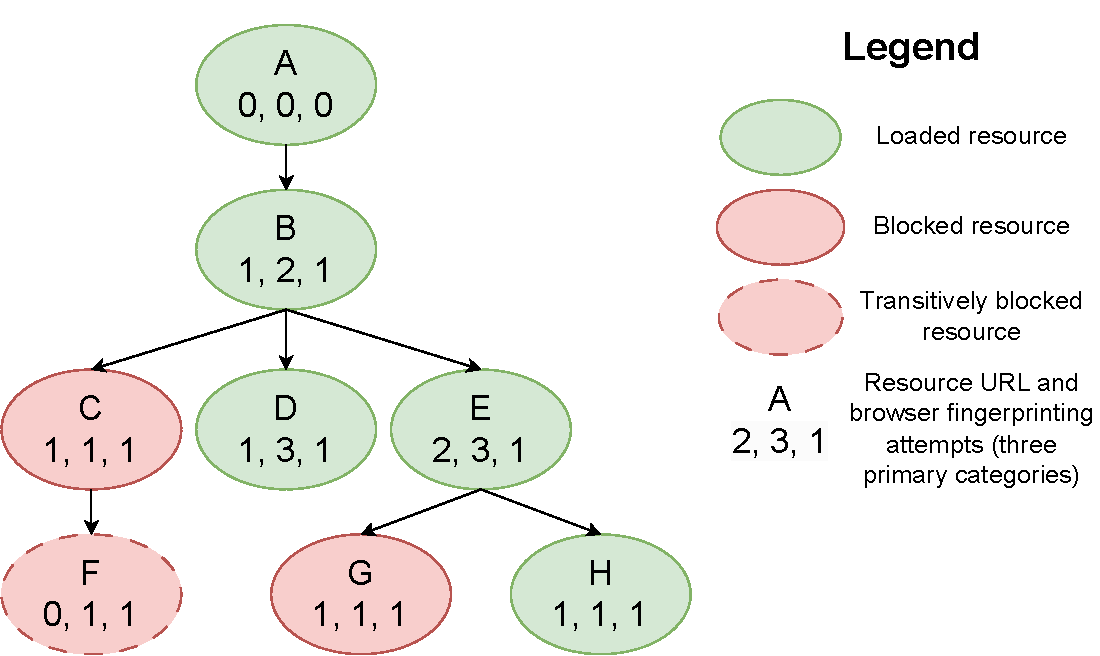
\includegraphics[width=\textwidth]{obrazky-figures/request_tree_visualization_better.drawio (1).pdf}
    \caption[Example request tree including multiple blocking situations]{Visualization of a~request tree with assigned fingerprinting API calls and block statuses as a~visual aid to explain the~measured metrics. Each node contains its URL (represented by a~single letter in the~node) and number of observed fingerprinting API calls, split into three primary categories as described in Subsection~\ref{fp-groups-apis}.}
    \label{request_tree_analysis_figure}
\end{figure}

\subsection{Requests Analysis}
\label{metrics-section}
For the~request blocking analysis, most metrics consist of only a~single number, with one exception. All 
the metrics are explained below in the~same format as in the~created results file.

\begin{description}
\item[requests\_observed]
This metric should be consistent for all tools tested on the~same dataset. It represents the~total number of requests that were observed in the~dataset. In Figure~\ref{request_tree_analysis_figure}, this metric corresponds to the~number of nodes, $8$.

\item[requests\_blocked\_directly] 
Directly blocked requests are those that were explicitly blocked by a~content-blocking tool. None of their parent nodes is blocked. This metric represents the~total number of such nodes in the~request tree -- in Figure~\ref{request_tree_analysis_figure}, it is $2$.

\item[requests\_blocked\_transitively]
Transitively blocked requests are those blocked due to any preceding parent node being blocked. Since the~parent was blocked, these requests would have never occurred if the~tested browser visited the~page. In Figure~\ref{request_tree_analysis_figure}, there is only one such node, \emph{F}, which was blocked because \emph{C}, its parent, was blocked. Thus, this metric would be $1$.

\item[requests\_blocked\_in\_total]
The sum of \textit{requests\_blocked\_directly} and \textit{requests\_{\linebreak}blocked\_transitively}. For figure~\ref{request_tree_analysis_figure}, this number is $3$.

\end{description}

The following metrics are experimental, meaning their results are not as easy to grasp as the~previous metrics. They primarily measure the~\textit{aggresiveness} of a~content-blocking tool, with more aggressive tools blocking parent requests before any child request can be loaded. The~metrics may help distinguish between similarly performing tools and quantify the~tool's aggressiveness.

\begin{description}

\item[blocked\_requests\_with\_followup\_requests]
This metric represents the~number of directly blocked requests that have at least \emph{one} child node associated, i.e., they were responsible for at least one follow-up request. In Figure~\ref{request_tree_analysis_figure}, there is only one node that was blocked that also has at least one child node -- node \emph{C}, making this metric $1$.

\item[average\_request\_block\_level]
The average request block level represents the~average level at which blocking occurred in the~tree. Only the~first block in each subtree is considered. The~root of the~tree is considered as level $1$. In Figure~\ref{request_tree_analysis_figure}, node \emph{A} would be level $1$, node \emph{B} would be level $2$, nodes \texttt{C, D, E} would be level $3$ and nodes \texttt{F, G, H} would be level $4$. Since only the~first blocked node in each subtree is taken into account, this number is counted from nodes \emph{C} and \emph{G}, which is $\frac{3 + 4}{2} = 3.5$. This metric is only counted for websites that include at least one blocked request.

\item[blocked\_subtrees\_data]
This metric is composed of five numbers. It describes blocking of primary \textit{subtrees} in the~request tree. In the~context of this metric, subtrees are defined by the~following procedure: A~given request tree is traversed until the~first node with at least \textit{two} child nodes is found. Each child node then serves as a~root of its primary subtree.

In Figure~\ref{request_tree_analysis_figure}, the~tree is traversed until node \emph{B} is reached. Since node \emph{B} has \textit{three} children, nodes \texttt{C, D} and \emph{E}, these child nodes are used as root nodes of three primary subtrees. Five numbers are measured as part of this metric:

\begin{description}
\setlength\itemsep{0em}
\item[subtrees\_fully\_blocked] The~number of primary subtrees blocked at the~root level. In Figure~\ref{request_tree_analysis_figure}, only subtree with root node \emph{C} is fully blocked, making this metric $1$.

\item[subtrees\_partially\_blocked] The~number of primary subtrees that include a\linebreak blocked node anywhere but at the~root level. In Figure~\ref{request_tree_analysis_figure}, only subtree composed of nodes \texttt{E, G} and \emph{H} is partially blocked since one of its nodes, the~node \emph{G} is blocked, making this value $1$.

\item[subtrees\_not\_blocked] The~number of primary subtrees with no blocked nodes. In Figure~\ref{request_tree_analysis_figure}, only subtree \textit{D} includes no blocked nodes. Thus, the~metric is $1$.

\item[subtrees\_in\_total] The~total number of primary subtrees observed. It is the~sum of the~three metrics above -- subtrees not blocked anywhere and those blocked partially or fully. In Figure~\ref{request_tree_analysis_figure}, this metric is $3$. This metric should be consistent for all tools evaluated on the~same dataset.

\item[trees\_with\_blocked\_root\_node] The~number of times the~whole request tree was blocked due to a~\textit{root} node being blocked. In this context, \textit{root} nodes mean those described in Subsection~\ref{root-nodes}. If any root node were blocked in a~tree, this metric for such a~tree would be $1$. No root blocking occurs in Figure~\ref{request_tree_analysis_figure}, making this metric $0$. However, if node \emph{A} or \emph{B} were blocked, this metric would be set to $1$, and all three primary subtrees would be considered fully blocked. If a~request tree was blocked because a~root node was blocked, the~page would be inaccessible, and the~user would be presented with an~error page. The~user must manually interact with the~error page to access such a~page.
\end{description}

\end{description}

\subsection{Fingerprinting Analysis}
\label{metrics-fpd-section}
The fingerprinting analysis consists of four metrics, listed in the~same format as in the~produced results file. As described in Subsection~\ref{fp-groups-apis}, the~fingerprinting API calls are split into three categories. Therefore, each fingerprinting metric is composed of three numbers, with each number describing the~corresponding category -- \textit{BrowserProperties}, \textit{AlgorithmicMethods} and \textit{CrawlFpInspector}.

\begin{description}
\item[fpd\_attempts\_observed]
This metric should be consistent for all content-blocking tools evaluated on the~same dataset. It represents the~total number of fingerprinting API calls observed across all pages in the~dataset. In  Figure~\ref{request_tree_analysis_figure}, this metric is the~sum of attempts logged for each category for each node -- $(7, 12, 7)$.

\item[fpd\_attempts\_blocked\_directly]
Directly blocked fingerprinting attempts represent the~fingerprinting API calls associated with nodes that were blocked directly, as described above. In Figure~\ref{request_tree_analysis_figure}, this metric is the~sum of fingerprinting API calls observed for nodes \emph{C} and \emph{G}, which is $(2, 2, 2)$.

\item[fpd\_attempts\_blocked\_transitively]
Transitively blocked fingerprinting attempts are the~API calls associated with transitively blocked nodes, as explained above. If a~parent node was blocked, none of its child nodes would be loaded, and their corresponding fingerprinting API calls would be prevented. In Figure~\ref{request_tree_analysis_figure}, this metric is $(0, 1, 1)$, which corresponds to the~\emph{F} node, which is the~only transitively blocked node.

\item[fpd\_attempts\_blocked\_in\_total]
The number of fingerprinting attempts blocked in total is the~sum of \textit{fpd\_attempts\_blocked\_directly} and \textit{fpd\_attempts\_blocked{\linebreak}\_transitively}. In Figure~\ref{request_tree_analysis_figure}, this metric is $(2, 3, 3)$.
\end{description}